\documentclass{article}
\usepackage[]{amsmath}
\usepackage{pgfplots}
\pgfplotsset{compat=1.18}
\usepackage{amssymb}
\usepackage[]{pxfonts}
\usepackage[english]{babel}
\usepackage{tikz}
\usepackage[]{cancel}

\title{Revisão Prova 1 de Cálculo II\\Milton Kist}
\author{Erickson Giesel Müller}
\begin{document}
	\maketitle
	
	\section{Conteúdos}
		\begin{enumerate}
			\item Integrais primitivas
			\item Integrais indefinidas
			\item Métodos de integração: Substituição e Integração por partes.
			\item Integração definida via somas de Riemann
			\item Teorema Fundamental do Cálculo
			\item Integração envolvendo funções trigonométricas
			\item Técnicas de integração
			\item Cálculo de áreas de figuras planas
			\item Cálculo de comprimento de arco de curva plana
			\item Cálculo de volumes de sólidos de revolução
			\item Cálculo de áreas de superfícies de revolução
		\end{enumerate}
	\newpage
	\section{Integrais Primitivas}
		Uma função $F(x)$ é considerada primitiva de $f(x)$ em um intervalo I se para todo $x \in I$ temos $F'(x)=f(x)$.
		\subsection{Propriedades}
			$$G'(x)=(F(x)+k)' = F'(x)+0=F'(x)$$
	\section{Integral Indefinida}
		Integral indefinida é aquela que não tem limite de integração.
		\subsection{Propriedades}
			\begin{equation}
			\int f(x).dx.K = K.\int f(x).dx
			\end{equation}
			\begin{equation}
			\int [f(x)+g(x)].dx = \int f(x).dx + \int g(x).dx
			\end{equation}
		\subsection{Integrais imediatas}
			\begin{enumerate}
				\item $\int dx = x+K$
				\item $\int x^-1.dx = \int \frac{1}{x}.dx = \ln x+K$ \\ \textit{Se fizermos a derivação do exemplo 4, dará uma constante}
				\item $\int \sin x . dx = -\cos x +K$
				\item $\int x^\alpha .dx = \frac{x^{\alpha+1}}{\alpha+1}+K$
			\end{enumerate}
		\subsection{Integrais de Multiplicação}
			$$\int [f(x).g(x)]'.dx = \int[f'(x).g(x)+f(x).g'(x)].dx$$
			$$f(x).g(x) = \int f'(x).g(x).dx + \int f(x).g'(x).dx$$
			$$\int f'(x).g(x).dx = f(x).g(x) - \int f(x).g'(x).dx$$
				$$u = g(x)$$
				$$du = g'(x).dx$$
				$$dv = f'(x).dx$$			
				$$v = f(x)$$
			
			
			Para resolver a integral $\int 2x. \sin x .dx$:
				$$u = 2x$$
				$$du = 2.dx$$
				$$dv = \sin x.dx$$
				$$v = -\cos x$$
			$$\int 2x. \sin x . dx = \int u . dv$$
			como $\int f'(x).g(x).dx = f(x).g(x)-\int f(x).g'(x).dx$:
			$$2x. - \cos x - \int ( - \cos x ).2.dx$$
			$$u.v- \int v.du$$
			$$\int \sin x.2x.dx = 2x. - \cos x - \int (- \cos x).2.dx$$
			$$I = -2x.\cos x +2.\sin x + K$$
			
		\subsection{Integração por Partes}
			$$\int x^2.e^x.dx$$
			$$u = x^2$$
			$$du = 2x.dx$$
			$$dv = e^x.dx$$
			$$v = \int e^x.dx = e^x$$
			$$I=\int u.dv$$
			$$\int x^2.e^x.dx = x^2.e^x-\int e^x.2x.dx$$
			$$=x^2.e^x-2\int x.e^x.dx$$
			Para o integrando $\int x.e^x.dx$ aplicamos a derivação por partes novamente.
			$$u = x$$
			$$du = 1.dx$$
			$$dv = e^x.dx$$
			$$v = e^x$$
			$$I = \int u . dv$$
			$$\int x.e^x.dx = x.e^x-\int e^x.dx$$
			$$\int x.e^x.dx = x.e^x-e^x$$
			Logo:
			$$\int x^2.e^x.dx = x^2.e^x-2[x.e^x-e^x]+K$$
			$$= e^x.[x^2-2x+x]+K$$
			Prova real:
			\begin{equation}
				[e^x.(x^2-2x+x)]'= e^x.(x^2-2x+2)+e^x.(2x-2)
				=e^x.x^2
			\end{equation}
			
	\section{Método de integração por substituição ou mudança de variável de integração}
		Sejam $F'(x)=f(x)$ e $g$ está contido no domínio de $F$, podemos definir a composição $F(g(x))$. Que segundo a regra da cadeia é resolvida por $F'(g(x)).g'(x)$
		Exemplo:
			$$F(g(x)) = sen(5x+2)$$
			$$[F(g(x))]' = \cos (5x+2).5$$
	\section{Integral Definida}
		Determine a área da região S limitada pelas curvas $y = x^2+1$; $y= 0$; $x=0$ e $x=2$.
		\begin{center}
			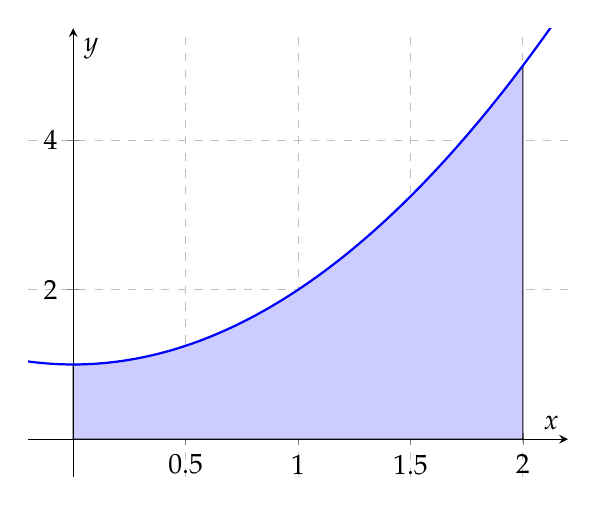
\begin{tikzpicture}
				\begin{axis}[
				    axis lines = middle,
				    xlabel = $x$,
				    ylabel = $y$,
				    ymin = 0,
				    xmin = 0,
				    xmax = 2,
				    ymax = 5,
				    grid = both,
				    grid style = dashed,
				    enlargelimits=0.1,
				    samples=500, % Aumentar o número de amostras
				]
					\addplot[fill=blue!20, domain=0:2] {x^2+1} \closedcycle;
					\addplot[color=blue, thick] {x^2+1}; % A função correta para a curva azul
				\end{axis}
			\end{tikzpicture}
		\end{center}
		A teoria para achar a área da seção é criar infinitos retângulos com base mínima e altura $f(x)$
		\subsection{Soma de Riemann}
			\begin{center}
				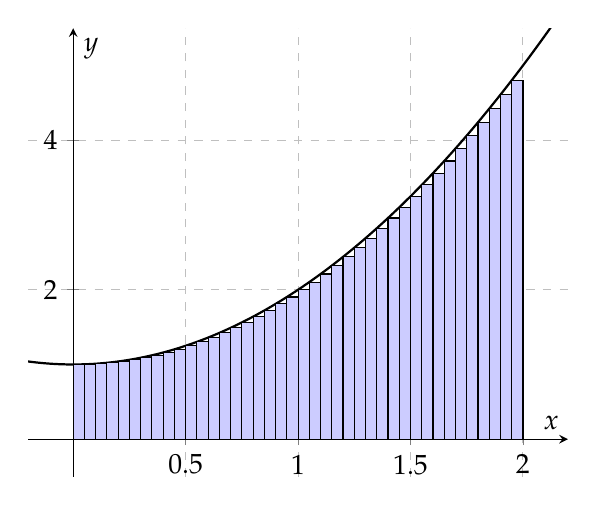
\begin{tikzpicture}
					\begin{axis}[
					    axis lines = middle,
					    xlabel = $x$,
				    	ylabel = $y$,
					    ymin = 0,
					    xmin = 0,
					    xmax = 2,
					    ymax = 5,
					    grid = both,
				    	grid style = dashed,
					    enlargelimits=0.1,
					    samples=500, % Aumentar o número de amostras
					]
						%\addplot[fill=blue!20, domain=0:2] {x^2+1} \closedcycle;
						\addplot[color=black, thick] {x^2+1}; % A função correta para a curva azul
						
						% Número de subintervalos (ajuste conforme necessário)
						\pgfmathsetmacro{\n}{10}

						% Largura de cada subintervalo
						\pgfmathsetmacro{\deltax}{0.05}

						% Loop para criar as colunas
						\foreach \i in {0,...,39}{
						    \pgfmathsetmacro{\x}{\i*\deltax} % Extremo esquerdo do subintervalo
						    \pgfmathsetmacro{\altura}{\x^2+1} % Altura da coluna
						    \addplot[fill=blue!20,thin,domain={\x:\x+\deltax}]{\altura} \closedcycle;
						    %\addplot[fill=blue!20, domain={\x}:\x+\deltax] {\x^2+1} \closedcycle;
						     
						}
					\end{axis}
				\end{tikzpicture}
			\end{center}
			Seja $P: a<x_1<x_2...<x_n=b$ uma partição uniforme do intervalo $[a,b]$. Dessa forma vamos construir $n$ retângulos de base $\Delta x = \frac{b-a}{n}$ e $h=f(C_i)$ onde $C_i \in (x_{i-1},x_i)$.\\
			Desta forma:
				$$A=f(C_1).\Delta x+f(C_2).\Delta x ... + f(C_i).\Delta x$$
				$$A = \Delta x.[f(C_1)...f(C_i)]$$
				$$A = \sum_{i=1}^{x}f(C_i).\Delta x$$
			Caso exista $\lim_{x \to \infty}A$, este será denominado integral de $x\to \infty$.
			Riemann (integral definida) da função $f$ é indicada por:
				$$\int_{a}^{b}f(x).dx = \lim_{x\to +\infty}\sum_{i=1}^{h}f(C_i).\Delta x$$
	\section{Teorema Fundamental do Cálculo}
		Seja $f[a,b]\to \mathbb{R}$ uma função contínua e $F$ uma primitiva de $f$. Nestas condições:
			$$\int_a^bf(x).dx = F(b)-F(a)$$
		exemplo:
			$$\int_0^2(x^2+1).dx=[\dfrac{x^3}{3}+x]_0^2=(\dfrac{2^3}{3}+2)-(\dfrac{0^3}{3}+0)=\dfrac{14}{3}$$
		\subsection{Demonstração}
			Seja $P: a=x_0<x_1...<x_n=b$ uma partição do intervalo $[a,b]$. Neste caso a Soma de Riemann da função $f$ é dada por:
				$$S_n=\sum_{i=1}^n f(C_i).(x_i-x_{i-1}),C_i \in [x_{i-1},x_i]$$
			Como $f$ é contínua, então, pelo \textbf{teorema do valor médio para derivadas}, temos que:\\
				Se $f$ é contínua em $[a,b]$ entãoexiste $C \in ]a,b[$ tal que:
				$$f'(C) = \dfrac{f(b)-f(a)}{b-a}$$
			Em cada intervalo $[x_{i=1},x_i]$ existe $C_i$ tal que:
				$$F'(C_i)=\dfrac{F(x_i)-F(x_{i-1}}{x_i-x_{i-1}}$$
				$$F'(C_i)=f(C_i)$$
			Logo:
				$$Sn= \sum_{i=1}^n \dfrac{F(x_i)-F(x_{i-1}}{\cancel{x_i-x_{i-1}}}.\cancel{(x_i-x_{i-1})}$$
				$$Sn = [F(x_1)-F(x_0)]+[(F(x_2)-F(x_1)]+...+[F(x_n)-F(x_{n-1})]$$
				$$Sn = -F(x_0)+F(x_n)$$
				$$Sn=F(b)-F(a)$$
			Como:
				$$\int_a^bf(x).dx = \lim_{n\to +\infty}Sn=\lim_{n \to +\infty}[F(b)-F(a)]$$
				$$=F(b)-F(a)$$
	\section{Integração Imprópria}
		Em intervalos finitos\\
		Se $f$ for contínua no intervalo $(a,b]$ e para todo $a<t<b$ existe a integral $\int_t^bf(x).dx$, então:
		$$\int_a^bf(x).dx = \lim_{t \to a^+} \int _t^bf(x).dx$$
		
		\begin{center}
			Desde que o limite exista em $\mathbb{R}$
		\end{center}
		
		Se $f$ for contínua no interval $[a,b)$ e para todo $a<t<b$ exista a integral $\int_a^tf(x).dx$, então:
		$$\int_a^bf(x).dx = \lim_{t \to b^-}\int_a^tf(x).dx$$
		\begin{center}
			Desde que o limite exista em $\mathbb{R}$
		\end{center}
		
		exemplo:\\
		Calcule a integral $\int_2^5\dfrac{1}{\sqrt[]{x-2}}$\\
		Domínio de $f$ é $(2,+\infty)$
		$$x-2>0 \to x>2$$
		$f$ é contínua no intervalo $(2,5]$. Seja $2<t<5$:
		$$\lim_{t \to 2^+} \int_t^5\dfrac{1}{\sqrt[•]{x-2}}.dx$$
		Sendo $u = x-2$ e $du = 1.dx$:
		$$I=\int u^{-\dfrac{1}{2}}.du = \dfrac{u^{-\dfrac{1}{2}}}{\dfrac{1}{2}}$$
		$$2\sqrt[•]{u}=2.\sqrt[•]{x-2}$$
		$$\lim_{t\to 2^+}(2\sqrt[•]{5-2}-2\sqrt[•]{t-2})=2\sqrt[•]{3}$$
%	\newpage
	\section{Métodos de Integração}
		\subsection{Integração de funções trigonométricas}
			\begin{enumerate}
				\item Determine $\int (2x-1).\sin(x^2-x).dx$:\\
					Considerando $u = x²-x$ e $du = (2x-1).dx$
					$$I = \int \sin u . du=-\cos (x^2-x)+c$$
				\item Determine $\int \tan x.dx$:\\
					$$\int \tan x .dx = \int \dfrac{\sin x}{\cos x}.dx$$
					Considerando $u=\cos x$ e $du = -\sin x$
					$$I = \int -u^{-1}.du=-\int -u^{-1}.du $$
					$$-\ln |u|+c=-\ln |\cos x| +c=\ln |\cos x|^{-1}+c$$
					\textit{Tentar entender por que $-\ln |\cos x| = \ln |\cos x|^{-1}$}\\
					\textit{Propriedade de Logaritmos $\log x^n = n.\log x$}
					$$I = \ln |\sec x|+c$$
				\item Determine $\int \cot x.dx$::
					$$\int \cot x.dx = \int \dfrac{\cos x}{\sin x}.dx$$
					Considerando $u = \sin x$ e $du = \cos x.dx$
					$$I = \int u^{-1}.du=\ln |u|+c = \ln |\sin x| + c$$
				\item Determine $\int x^2.\cot x^3.dx$:\\
					Considerando $u = x^3$ e $du = 3x^2.dx$
					$$I = \int \cot u . \dfrac{du}{3}=\dfrac{1}{3}.\ln |\sin x^3| + c$$
				\item Determine $\int \sec x.dx$:\\
					$$\int \sec x.dx = \int \cos^{-1} x.dx$$
					Considerando
			\end{enumerate}
\end{document}